\chapter{Data Collection and Processing}

We outline the process of collecting, storing, and preprocessing all of the price data and
alternative textual data used in our trading strategies.
Implementations for each part can be found on our project GitHub repository.

\section{Data Sourcing}

\subsection{Stock Price Data}
The BUFN Computational Finance Minor program provided us with access to Wharton Research Data Services (WRDS),
an in particular, data from the Center for Research in Security Prices (CRSP).
Pursuant to the ideas and implementation of \cite{drl_framework}, we downloaded basic stock price data (close/high/low price, volume, and metadata)
for all stocks in the S\&P100 index from 2010 to 2020. We also downloaded data for the S\&P500 value-weighted and equally-weighted indices for benchmark comparison.

\subsection{News Data}

\subsubsection{Scraping Attempts}
While attempts have been made to scrape news data from financial sources including Yfinance and Benzinga,
we have primarily been rate limited/and or IP blocked for scraping at too high of a frequency.
There exist some APIs that provide real-time and historical news data pipelines for business and professional 
use, including Event Registry, newsapi.ai, and Alpha Vantage provide 
this data. However, all of them require a significant payment to get data at a velocity 
that we would need, and historical data is often even more expensive.
While some have a free tier that allows for limited data collection, it is not sufficient
in quantity or scope for our purposes.

\subsubsection{News Headlines Dataset}
The dataset we use in this project is Daily Financial News for 6000+ Stocks that was downloaded via Kaggle \cite{financial_news}.
This dataset contains scraped headline data for over 6000 stocks listed on the NYSE exchange from 2009-2020. 
There are two main files within this dataset that we use. The first is \texttt{raw\_analyst\_ratings.csv}, which only contains scraped data from a prominent financial news publisher Benzinga.
The other file \texttt{raw\_partner\_headlines.csv} contains scraped headline data from other smaller publishers that partner with Benzinga. Each row of the datasets contains a headline, the base article URL, the date and time of publication, and the stock ticker symbol.
The \texttt{raw\_analyst\_ratings.csv} file does not contain publisher information, as it is already implied that Benzinga is the publisher. Meanwhile, the table in \texttt{raw\_partner\_headlines.csv} has a column indicating the publisher of each article. 
We concatenate the headline data from each file to create a single unified dataset that contains all headlines for each stock in our universe.

\subsection{SEC Data}
We used the EDGAR database to downloaded 10-K and 10-Q SEC filings for most companies in the S\&P100 for the last 30 years.
The results are a set of HTML files taking up roughly 115GB of storage space, which we stored in Google drive.
We built parsers to extract the key sections from both types of filings; in particular, Item 7/7A from the 10-K and Item 2 from the 10-Q.
This is the Management’s Discussion and Analysis (MD\&A) section, which allows the company management to discuss
"the company’s exposure to market risk, such as interest rate risk, foreign currency exchange risk, commodity price risk or equity price risk,", and "how it manages its market risk exposures" \cite{sec_how_to_read_10kq}.



\section{News Data Processing}

\subsection{FinBERT Sentiment Scores}\label{finbert}

Over the full trading period (2010-2020), we will feed all of the headlines and selected SEC filings text for S$\&P$ 100 companies to pre-trained FinBERT. 
The model then generates probabilities of the content having a positive, negative, or neutral sentiment. For the news headlines, we developed a novel function to extract a single embedding for a stock on a given day. 

The function that we created is:
\begin{equation}\label{eq:value_embedding}
  \texttt{Value}_{\texttt{Embedding}} = \tanh\Biggl( \frac{\frac{\texttt{positive sentiment probability}}{\texttt{negative sentiment probability}}}{\texttt{neutral sentiment probability}} \Biggr)
\end{equation}
This approach combines the “log likelihood” (ratio of probabilities of positive and 
negative sentiment) along with a penalty for high neutral sentiment (a measure of 
uncertainty), using the tanh for normalization. This approach would allow us to 
adequately detect strong positive/negative sentiment. Thus, a sentiment score close to 1 can be interpreted as a positive sentiment, a score close to 0 can be interpreted as neutral, and a score close to -1 can be intepreted as negative.

An issue that we run into when incorporating SEC filings data is that they are recorded on a annual or quarterly basis, which is far more infrequent than our samples for price and news data.
Thus, to fill the gaps between SEC filings dates, we apply exponential decay to the sentiment scores on report dates. Formally,
\begin{equation}\label{eq:sentiment_deday}
  y = a(1 - \gamma)^t
\end{equation}
Where $a$ represents the company's sentiment score on the most recent reporting date,
$t$ represents time (in days) between the last report date and the current day,
and $\gamma$ is a constant between 0 and 1 representing the daily decay factor.
We test $\lambda = 0.1, 0.5, 0.9$ in our models to see what performs optimally. Note that we test a wide range of $\gamma$ values because we are unsure of how fast the signal from SEC filings decay. We also run experimented with using this same routine to fill some gaps between news data.

\subsection{Creating News Tensors}\label{newstensors}

From the concatenated dataset of news headline data from each publisher as described in the "News Data" section, we feed the dataset (loaded into a pandas dataframe) through a multi-stage pipeline. 
The first step is to scrape the current S\&P 100 companies and then filter the dataset down to only include headlines from companies in the S\&P 100. 
We introduce a custom dataset class called "NewsHeadlines," implemented in PyTorch framework, designed for efficiently handling news headline data. 
The class takes a dataset and a user-defined tokenizer which will pre-process headlines in batches to be fed into FinBERT. 
In the class, we implement an iterator function \texttt{\_getitem}, which takes the raw headline data as input and returns an encoding for the batch of headlines after tokenization. 
Then given the large size of the dataset, we use a create a "Dataloader" object, implemented in PyTorch, which feeds our dataset into the model in small batches. 

To obtain the output tensors corresponding to the sentiment probabilities, we iterate over the batches, applying FinBERT to classify each headline and from the raw logits using the softmax activation function to a vector of probabilities.
Then for each batch, we save off the tensors to separate files. A finalized version of this process is available in \texttt{utilities\\news\_data\_processing.py}
Then in the \texttt{tensor\_data\_loading.ipynb} script, we merge the tensors with the original concatenated dataset and create our the sentiment embedding as described in the "FinBERT Sentiment Scores" section. 
This finalized dataset is then written to \texttt{news\_sentiment\_data.csv}.

\subsection{News Dataset Statistics}\label{newsstats}

Our dataset contains data for 84 out of the total 100 tickers in the $S\&P$ 100,
and it contains 70,872 entries containing the sentiment embedding of news for a company on a given day.
Table \ref{table:news_dist} displays some  summary statistics on the distribution of news reports across the tickers.

\begin{table}[htbp]
    \centering
    \caption{Company News Reporting Date Distribution}
    \begin{tabular}{l c}
        \toprule
        \textbf{Statistic} & \textbf{Value} \\
        \midrule
        Count & 84 \\
        Mean No. of Reporting Dates & 843.714 \\
        Standard Deviation & 508.209 \\
        Minimum Observations & 1 \\
        25th Percentile & 393.250 \\
        Median & 905.000 \\
        75th Percentile & 1198.500 \\
        Maximum & 1829 \\
        \bottomrule
    \end{tabular}
    \label{table:news_dist}
\end{table}

Note that given our median ticker only has news reports on 905 of the total trading dates and because there are 16 tickers for which we have no sentiment data, our dataset is still suboptimal for developing an agent. Our forward filling process, does address some of the gaps in our data, however our coverage is still not complete.
This is an important consideration when examining the results of our work.

\begin{figure}
  \centering
  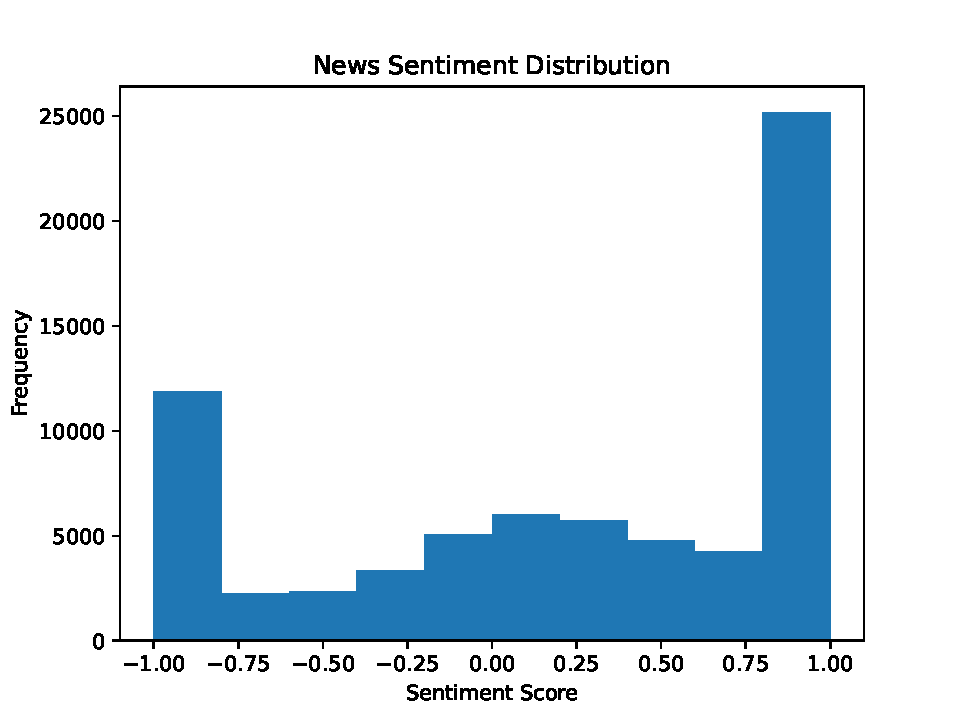
\includegraphics[width=.9\textwidth]{../figures/news_sent_dist}
  \caption{Frequency distribution of our novel news sentiment scores.}
  \label{fig:news_dist}
\end{figure}

Figure \ref{fig:news_dist} shows the distribution of sentiment scores across the articles.
News sentiment has a bimodal distribution: much of the headlines are interpreted as either negative or positive, but news headlines that are relatively neutral, or closer to 0, or more evenly distriubuted. 
This indicates that the headlines that display strong enough sentiment that they could inform and change the actions of our reinforcement learning agents.



\section{SEC Data Processing}

\subsubsection{Creating SEC Tensors}
To extract meaningful values from the text, we first parse and clean the SEC filing HTML documents so we can extract the raw text.
Then we use regular-expression based text parsing to extract text from Item 1A and 7/7A, and Item 2 in 10-Qs.
We then construct a data frame, where each row contains the company ticker, the date of the filing, the extracted section name, the text of the extracted section.
We then pass this into the FinBERT model to add a final column containing sentiment scores, calculated by the methodology explained in Section \ref{finbert}.
However, issues were encountered both with the size of the dataset being computationally intensive, along with parsing issues due to the way the filings are stored and transmitted.
The process to create SEC-sourced tensors is then to extract positive, negative, and neutral words as specified by the Loughran-McDonald sentiment dictionary.
We then utilize the proportions in a similar fashion to the news embeddings using Equation \eqref{eq:value_embedding}.

\subsubsection{SEC Filings Dataset Statistics}
Our dataset contains data for 99 out of the 100 tickers in the S\&P 100, containing over 9,000 filings between 1994 and the present day, with the used subset consists of roughly 6,100 filings.
Table \ref{table:sec_dist} shows some reported summary statistics on the distribution of SEC filings across the tickers:

\begin{table}[htbp]
    \centering
    \caption{Company SEC Filings Distribution}
    \begin{tabular}{l c}
        \toprule
        \textbf{Statistic} & \textbf{Value} \\
        \midrule
        Count & 99 \\
        Mean No. of Filings & 61.42 \\
        Standard Deviation & 10.18 \\
        Minimum Observations & 20 \\
        25th Percentile & 64 \\
        Median & 65 \\
        75th Percentile & 65 \\
        Maximum & 66 \\
        \bottomrule
    \end{tabular}
    \label{table:sec_dist}
\end{table}

Since there are only 4 filings per year, we use forward filling with decay to fill in the "missing" dates.
Giving the addition and dropping of companies from the S\&P100, as well as some newer public companies joining, each company does not have the same number of filings over the time period.

\begin{figure}
  \centering
  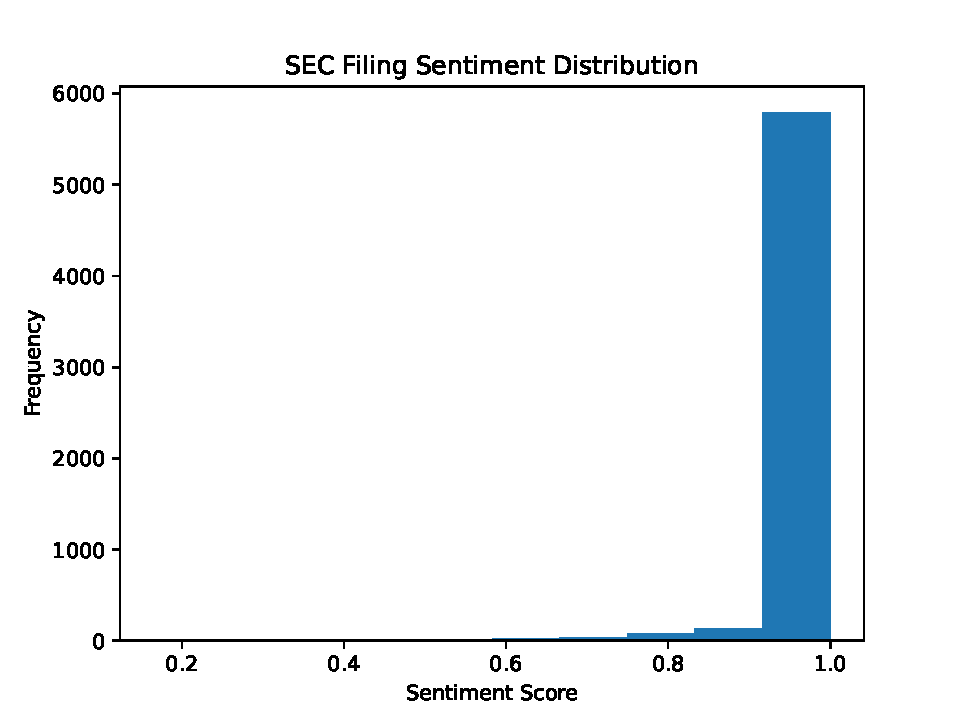
\includegraphics[width=.9\textwidth]{../figures/sec_sent_dist}
  \label{fig:sec_dist}
\end{figure}

Figure \ref{fig:sec_dist} shows the distribution of sentiment scores.
There is a pronounced tail towards 1, indicating a strongly positive unimodal distribution, as compared to that of the news sentiment.
Since we utilize sections of the SEC filings that are written by the companies themselves,
it is likely that companies aim to provide filings that suggest strong performance and future outlook.
In the dataset, we do observe some drops in sentiment, such as times of financial crisis or bad market conditions, like in 2013 for some technology-based companies.


